\documentclass[aps,prl,twocolumn,groupedaddress]{revtex4-1}
% \documentclass[aps,twocolumn,secnumarabic,balancelastpage,amsmath,amssymb,nofootinbib]{revtex4-1}
\usepackage{amsmath}
\usepackage{amssymb}
\usepackage{amsfonts}
\usepackage{color}
\usepackage{graphics}
\usepackage[pdftex]{graphicx}
\usepackage[utf8x]{inputenc}
\usepackage[colorlinks=true]{hyperref}

\newcommand{\ud}{\mathrm{d}}
\newcommand{\ue}{\mathrm{e}}
\newcommand{\ui}{\mathrm{i}}
\newcommand{\res}{\mathrm{Res}}
\newcommand{\Tr}{\mathrm{Tr}}
\newcommand{\dsum}{\displaystyle\sum}
\newcommand{\dprod}{\displaystyle\prod}
\newcommand{\dlim}{\displaystyle\lim}
\newcommand{\dint}{\displaystyle\int}
\newcommand{\fsno}[1]{{\!\not\!{#1}}}
\newcommand{\texp}[2]{\ensuremath{{#1}\times10^{#2}}}
\newcommand{\dexp}[2]{\ensuremath{{#1}\cdot10^{#2}}}
\newcommand{\eval}[2]{{\left.{#1}\right|_{#2}}}
\newcommand{\paren}[1]{{\left({#1}\right)}}
\newcommand{\lparen}[1]{{\left({#1}\right.}}
\newcommand{\rparen}[1]{{\left.{#1}\right)}}
\newcommand{\abs}[1]{{\left|{#1}\right|}}
\newcommand{\sqr}[1]{{\left[{#1}\right]}}
\newcommand{\crly}[1]{{\left\{{#1}\right\}}}
\newcommand{\angl}[1]{{\left\langle{#1}\right\rangle}}
\newcommand{\tpdiff}[4][{}]{{\paren{\frac{\partial^{#1} {#2}}{\partial {#3}{}^{#1}}}_{#4}}}
\newcommand{\tpsdiff}[4][{}]{{\paren{\frac{\partial^{#1}}{\partial {#3}{}^{#1}}{#2}}_{#4}}}
\newcommand{\pdiff}[3][{}]{{\frac{\partial^{#1} {#2}}{\partial {#3}{}^{#1}}}}
\newcommand{\diff}[3][{}]{{\frac{\ud^{#1} {#2}}{\ud {#3}{}^{#1}}}}
\newcommand{\psdiff}[3][{}]{{\frac{\partial^{#1}}{\partial {#3}{}^{#1}} {#2}}}
\newcommand{\sdiff}[3][{}]{{\frac{\ud^{#1}}{\ud {#3}{}^{#1}} {#2}}}
\newcommand{\tpddiff}[4][{}]{{\left(\dfrac{\partial^{#1} {#2}}{\partial {#3}{}^{#1}}\right)_{#4}}}
\newcommand{\tpsddiff}[4][{}]{{\paren{\dfrac{\partial^{#1}}{\partial {#3}{}^{#1}}{#2}}_{#4}}}
\newcommand{\pddiff}[3][{}]{{\dfrac{\partial^{#1} {#2}}{\partial {#3}{}^{#1}}}}
\newcommand{\ddiff}[3][{}]{{\dfrac{\ud^{#1} {#2}}{\ud {#3}{}^{#1}}}}
\newcommand{\psddiff}[3][{}]{{\frac{\partial^{#1}}{\partial{}^{#1} {#3}} {#2}}}
\newcommand{\sddiff}[3][{}]{{\frac{\ud^{#1}}{\ud {#3}{}^{#1}} {#2}}}
\newcommand{\eff}{ef\! f}
\newcommand{\fxnote}[1]{{\textbf{[#1]}}}

\newcommand{\todo}[1]{}

\ifpdf
% Ensure reproducible output
\pdfinfoomitdate=1
\pdfsuppressptexinfo=-1
\pdftrailerid{}
\hypersetup{
  pdfcreator={},
  pdfproducer={}
}
\fi

\begin{document}
\title{Coherent optical association of single molecules}
\author{Yichao Yu}
\email{yichaoyu@g.harvard.edu}
\author{Kenneth Wang}
\author{J. D. Hood}
\author{Lewis Picard}
\author{Jessie T. Zhang}
\author{William Cairncross}
\author{Jeremy Hutson}
\author{Till Rosenband}
\author{Kang-Kuen Ni}
\email{ni@chemistry.harvard.edu}
\affiliation{Department of Chemistry and Chemical Biology, Harvard University, Cambridge, Massachusetts, 02138, USA}
\affiliation{Department of Physics, Harvard University, Cambridge, Massachusetts, 02138, USA}
\affiliation{Harvard-MIT Center for Ultracold Atoms, Cambridge, Massachusetts, 02138, USA}

\date{\today}

\begin{abstract}
  We report on coherent association of a single weakly-bound NaCs molecule in an optical tweezer
  through an optical Raman transition without the use of a Feshbach resonance. Our scheme borrows transition dipole moment while reducing photon scattering by selecting a deeply bound electronic excited intermediate state.
  Starting from two atoms in their relative motional ground state,
  we achieve optical transfer efficiency of $50 \%$ \todo{number}.
  The molecule has a (change to 8.8G) zero-field binding energy of $770 \mathrm{MHz}$ \todo{number}
  and lifetime up to $1 \mathrm{ms}$ \todo{number}. (center of mass motional state population.)
  %We demonstrate that coherent creation of a ground-state single molecule is possible, even without Feshbach resonance or narrow optical transition.
  This  technique is general (does not rely on narrow excited state linewidth) and could allow a wider range of molecular species to be assembled atom-by-atom.
\end{abstract}

% Coherent
% Intermediate state
% Motional state control
% Initial state preparation

\maketitle

% Introduction

Trapped neutral molecules, assembled in an array of optical tweezers, are a promising platform to study quantum infoqrmation and quantum simulations.
1. we want to have a diverse species to tailor to different applications. 2. but so far all has been done with Feshbach association (before STIRAP), or in the case of Sr2, a narrow excited state. Previous work on near-threshold Raman transfer has been incoherent. (suggested referees: Florian Shreck and Immanual Bloch)

In this Letter, we survey theoretically the best electronic intermediate state, detuning, etc that balance coupling/transfer efficiency and photon scattering to demonstrate coherent association of a electronic ground-state molecule from two atoms. Because the electronic excited state we used are generic in most diatomic molecules, this technique is general....


\begin{figure*}
  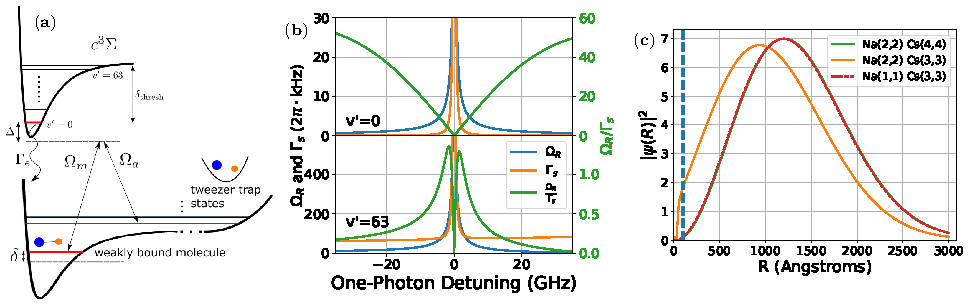
\includegraphics[height=4.5cm]{fig1.pdf}
  \caption{Optical creation of single molecule from single atoms in tweezer.
    (A) Schematics of the Raman transition. \todo{more about the states involved}
    (B) Geometry and polarization of trap and Raman beam relative to the bias magnetic field.
    \todo{Field strength, power, polarization description (pi)}
    (C) Molecule formation pulse sequence. The tweezer initially consists of only up leg power.
    This power is smoothly ramped down and the down leg power ramped up over $10\mu s$ while
    maintaining the total power of the tweezer.
    \todo{to minimize heating?}
    \label{f-setup}
  }
\end{figure*}

\begin{figure*}
  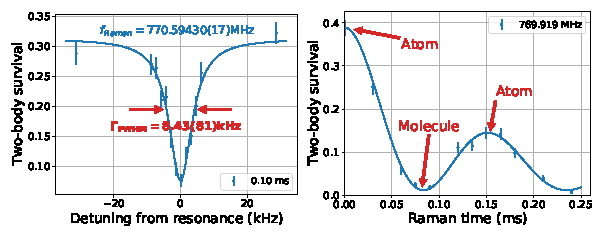
\includegraphics[height=4.5cm]{fig2.pdf}
  \caption{
    (A) Raman resonance from atomic state to molecular state, showing Fourier limited linewidth.
    \todo{states, time}
    (B) Rabi oscillation on resonance
    \label{f-raman}}
\end{figure*}

\begin{figure*}
  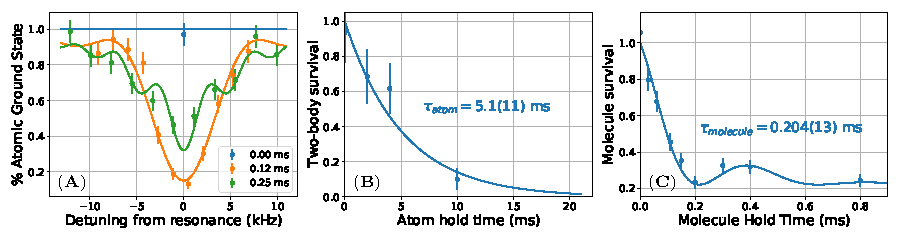
\includegraphics[height=4.5cm]{fig3.pdf}
  \caption{
    (A) Molecule lifetime in 15 mW of trap depth \todo{lifetime number}
    (B) Two-body atom lifetime in 15 mW of trap depth \todo{lifetime number,
      subtraction of single body, photoassociation rate}
    \label{f-lifetime}}
\end{figure*}

\begin{figure*}
  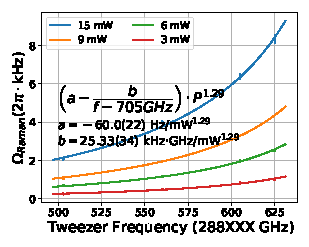
\includegraphics[height=4.5cm]{fig4.pdf}
  \caption{Raman Rabi frequency vs detuning
    \label{f-det}}
\end{figure*}

\todo{Previous result}
\todo{talk about size mismatch, two step transfer/weakly bound molecule in intro}

For atoms in the motional ground state in the tweezer, the average distance between the two atoms is $...$. However, for the ground rovibrational molecule, the bond length is only $...$. The size mismatch between the initial and final state causes a very small wavefunction overlap between the initial and final state, \todo{overlap is always 0, the accurate description here is the product of wavefunction overlap through any reasonable intermediate state, or the density-density correlation which serves as a reasonable estimate of the matrix element through different pathways} which poses the biggest challege for for coherent creation of the molecule. Because of this, it is necessary to use a intermediate state with a size in between the initial and final state and accomplish the transfer in two steps, each with improved wavefunction overlap.

The traditional choice for such an intermediate state is a FB molecule \todo{cite our FB result}. However, the requirement of a suitable FB resonance limits its generality (e.g. non-magnetic atoms). Instead, we selected a weakly bound molecular state as the intermediate state and we use an optical Raman transition as the first step transfer. This approach relies on fewer special properties of the system and can be more generally applied to creating other molecules. Such a transfer using optical transition has been observed in previous experiments (\todo{cite}). However, they either require the use of a narrow optical transition which limits the generality or were driving the transition incoherently due to scattering. In this letter, we will present our result on coherent creation of a weakly bond molecule using only optical transition for the first time.

Even with the first step transfer to a weakly bond molecular state, it is still a challenge to achieve high enough Raman Rabi frequency to drive this transition due to the wavefunction size mismatch with the excited molecular state. For this reason, previous experiments also use weakly bond molecular excited states for the Raman transition. However, for a typical molecular potential, vibrationally excited states have a smaller spacing between neighboring states which limits the detuning for the Raman transition and increases the scattering. Moreover, there is also a significant scattering process from the excited atomic states due to the strong coupling with the weakly bond molecular ground state. Such scattering process is proportional to $1/\delta^2$ from the desociation threshold which is also much stronger for more weakly bound states. (combining these factors, confirm with figure 1 Rabi rate vs scattering rate calculation). Because of this, we use a deeply bound molecular excited state to drive the Raman transition.

(mention scattering/lightshift depends on up/down matrix element ratio?)

In additional to the final and the excited state, it is also important to select the an initial atomic state in order to improve the coupling. Due to the small size of the molecular wavefunction, the coupling between the ground atomic state and the excited molecular state is approximately proportional to the value of the relative atomic wavefunction at short distance. In additional to the confinement, this value is related to the interaction between the two atoms. States with a large scattering length (positive or negative), the phase shift in the relative wavefunction between the atoms can significantly increase the short range wavefunction (add figure?). The increase in the coupling is proportional to (quote/cite Olive's equation?).
For our system, among the stable spin combinations, 4422 and 3311 has a small scattering length of $\abs{a}=....$ respectively and 3322 has a large and negative scattering length.
(interaction shift $\approx$ binding?)

%% Preparation
Our experiment begins by loading a single ${}^{23}\mathrm{Na}$ atom and a single ${}^{133}\mathrm{Cs}$ atom into an optical tweezer from a dual-species MOT\todo{cite na loading paper} into separate optical tweezers. The atoms are imaged to distinguish between loading of two atoms, one atom (Na or Cs), or no atom during post selection. We then perform simutanious Raman sideband cooling (RSC) to cool both atoms into a single 3-dimentional motional ground state in the tweezers. After RSC, the Na tweezer is moved by sweeping the frequency on an acustical optical beam deflector (AOBD) to overlap with the Cs tweezer before smoothly ramping off so that the Na and Cs atoms are merged into the same tweezer \todo{cite}. The spin states for the Na and Cs atoms after RSC and during the merge process are $|F=2,m_F=2\rangle$ and $|F=4,m_F=4\rangle$ respectively. This states combination has a low scattering length of $... a_0$ which allows the two atoms to be merged into the same tweezer with minimum pertubation on each other and remains in their motional ground state after the merge.

After preparing the Na and Cs atoms in the same tweezer in a single quantum state, we perform interaction shift spectroscopy using a Cs Raman transition to drive the Cs into the $|F=3,m_F=3\rangle$ state. The new spin state combination has a larger scattering length of $... a_0$ which generates a interaction shift of $... kHz$ in the tweezer. This interaction shift is larger than the differential axial trapping frequency between Na and Cs atoms, which decouples the relative and center of mass motional state and improves the robustness of our preparation of relative motional ground state. The stronger interaction in this spin state also enhances the atomic wavefunction at short range and increases its overlap with the intermediate molecular state used for our Raman transfer.

%% Transfer scheme


The optical transfer scheme we used is shown in figure \todo{}.
We use an optical Raman transition to drive the system from the atomic initial state to a
ground electronic molecular state. In order to reduce the size mismatch between the atomic and molecular states,
we selected the first bound state for the 3322 spin state \todo{asymtopt to the 3322 threshold?} as our final state. \todo{move selection of intermediate state to intro?}.
For similar reason, the natural choice for the intermediate excited molecular state is one
with highly excited motional level.
However, from our calculation (and experiment?), the smaller level space for high
vibrational state and the smaller detuning from the atomic threshold increases the
the scattering rate of the molecular state which causes a reduced Raman Rabi frequency
to decoherence rate ratio and a lower transfer efficiency.
Therefore, in our experiment, we selected the v=0 state as the intermediate state for our
Raman transition.

The pulse sequence for the experiment can be seen in figure (). Instead of adding another beam to drive the Raman transition on the atoms in the tweezer, we use the tweezer itself to achieve this goal. After the total tweezer power is set to the desired value, we smoothly ramp down the power of one frequency in the tweezer while simutaniously ramping up the power of a different frequency so that the total tweezer power remains unchanged. Both frequencies are kept on for a variable length of time before the process is reversed and we return to having a single frequency in the tweezer. The dual use of the tweezer beam ensures that there is not any undesired laser frequency that can interfere with the Raman transition. Using the tweezer beam for the Raman transition also allow us to maximize the intensity of the Raman beams and minimize the transfer time.
\todo{clarify coprop of Raman beam?}

Figure () shows the geometry of the experiment setup. A $8.8\mathrm{G}$ B field was used to defines the quantization axis in the experiment and is applied perpendicular to the tweezer axis. The tweezer beam (both frequencies for the Raman transition) has a $\pi$ polarization relative to the quantization axis, which allows us to selectively drive the Raman transition to a final state with the same total $m_F$ quantum number as our initial state.

%% Prediction

This excited state used in the Raman transition was measured in our previous experiment using photoassociation to be at $288... GHz$ from our atomic state. The ground molecular state has not been observed previously in experimentally. Based on our measurement of FB resonance, interaction shift and the binding energy of the 4422 bound state. Theory prediction was at $770... MHz$. \todo{more, mention/cite Jeremy}

%% Experiment condition/resonance

We locate the Raman resonance for the atom to molecule transition at $770... MHz$ (figure \todo{}) with a $15 mW$ tweezer at $288... GHz$ which corresponds to a $... GHz$ single photon detuning.
The background level of $...\%$ corresponds to the propability of preparing the two atoms in the relative motional ground state using interaction shift spectroscopy. When the atoms are transfered into molecule by the Raman transition, there is a decrease in the two body survival since the resulting molecule is not directly detected by our imagine step.
\todo{more explanation of detection?}
\todo{FWHM of line??}

B field dependency $... kHz/G$ which agrees with theory prediction of $... kHz/G$.
Dependency on tweezer power $... kHz/mW$, extrapulated to obtain the bare resonance at $0$ tweezer power to be at $... MHz$.

After confirming the creating of the molecule via optical Raman transition, we proceed to verify the coherence of the process. This is done by fixing the Raman frequency on the resonance and scanned the pulse time. figure ... shows the observed Rabi oscillation between the atomic and molecular states. Fitting the data with a decaying Rabi oscillation suggests that $..\%$ of initial ground state atoms are transfered into the molecular state.

\todo{Atomic lifetime}

Combining the frequency and time scan allow us to accurately fit the parameters for the Raman transition.
Raman Rabi frequency
Molecular state lifetime.
The result shows that the decoherence of the Rabi oscillation is caused by finite lifetime of the molecule in the tweezer.
We can directly measure this by \todo{pulse sequence} (figure ...)...

\todo{Lifetime}

\todo{Fitting}

\todo{Scattering}

\todo{sm: STIRAP vs Raman}

\bibliography{paper}
\end{document}
